\documentclass[sustainability,article,submit,moreauthors,pdftex]{mdpi}

%=================================================================
% MDPI Journal Settings
%=================================================================
\firstpage{1} 
\makeatletter 
\setcounter{page}{\@firstpage} 
\makeatother
\pubvolume{1}
\issuenum{1}
\articlenumber{0}
\pubyear{2024}
\copyrightyear{2024}
%\externaleditor{Academic Editor: Firstname Lastname}
\datereceived{ } 
\daterevised{ } 
\dateaccepted{ } 
\datepublished{ } 
%\datecorrected{}
%\hrefterms{http://creativecommons.org/licenses/by/4.0/}

%=================================================================
% MDPI Title & Authors
%=================================================================
\Title{Policy Attention versus Institutional Supply: How Local Governments Foster Cluster Resilience---A Mixed-Methods Case Study of China's Gaoyang Textile Industry}

\Author{Yiwen Sun $^{1}$, Yanlin Shi $^{2,}$*, Jiarui Liang $^{1}$}

\AuthorNames{Yiwen Sun, Yanlin Shi, Jiarui Liang}

\address{%
$^{1}$ \quad School of Mathematics and Statistics, Beijing Technology and Business University, Beijing, China; yver\_sun@163.com\\
$^{2}$ \quad School of Languages and Communication, Beijing Technology and Business University, Beijing, China}

\corres{Correspondence: shiyanlin@th.btbu.edu.cn}

%=================================================================
% Abstract & Keywords
%=================================================================
\abstract{
Traditional labor-intensive industrial clusters in developing economies face existential threats from compounding environmental, trade, and technological shocks, yet the micro-level institutional mechanisms through which local governments foster cluster adaptability remain undertheorized. This study advances a conceptual distinction between \emph{policy attention} (discursive emphasis in official documents) and \emph{institutional supply} (actual resource allocation), and traces two sequential micro-mechanisms---compliance cost socialization through collective environmental infrastructure, and transaction cost reduction through e-commerce and regional branding---through a 25-year (2000--2024) mixed-methods case study of China's largest towel production cluster in Gaoyang County. We combine BERTopic dynamic topic modeling of government work reports with descriptive quantitative patterns from Synthetic Control Method (SCM) and Interrupted Time Series (ITS) analysis. The case reveals a two-stage resilience trajectory: environmental infrastructure investment secured \emph{baseline resilience} during the 2017 regulatory shock, while subsequent digital and branding policies fostered \emph{value resilience}. Quantitative patterns are directionally consistent with the theoretical framework but, given single-case constraints and limited statistical power, are properly interpreted as mechanism-illustrative rather than causal-confirmatory. The paper contributes a portable conceptual framework for distinguishing policy signals from institutional actions, a microeconomic formalization of compliance cost and transaction cost channels, and a transparent template for mixed-methods policy evaluation under archival data constraints.
}

\keyword{Regional Economic Resilience; Sustainable Development; Dynamic Topic Modeling; Synthetic Control Method; Industrial Clusters; Environmental Regulation; Textile Industry; China}

\begin{document}
\section{Introduction}\label{sec:intro}

The global economic landscape has shifted from hyper-globalization to an era of \emph{polycrisis} \citep{Tooze2021}. Traditional labor-intensive industrial clusters in developing economies confront overlapping shocks---environmental regulation, trade friction, and technological disruption---that pose existential threats to their sustainable development \citep{Gong2022, Zhou2017}. Some clusters collapse under these pressures, while others demonstrate remarkable adaptability, successfully upgrading their value chains while meeting strict environmental standards. This divergence raises a critical question: How do traditional industrial clusters construct and evolve resilience under compounding shocks, and what role does local government policy attention play in balancing economic survival with environmental sustainability?

Regional Economic Resilience (RER) has become a central concept in economic geography and sustainability studies \citep{Martin2012, Boschma2015, Martin2015}. However, two gaps persist. First, empirical studies predominantly focus on advanced manufacturing clusters in developed nations, leaving traditional clusters in developing economies understudied \citep{Zhu2022}. Second, macro-level econometric analyses often treat institutional mechanisms as a \emph{black box}, neglecting how specific policy mixes evolve in response to shocks \citep{Grillitsch2020, Hassink2019}. Recent scholarship calls for more granular approaches that trace micro-level transmission mechanisms between policy interventions and sustainable firm outcomes \citep{RodriguezPose2013, HuHassink2017}.

We address these gaps through a mixed-methods longitudinal case study \citep{Creswell2017} of the Gaoyang towel cluster in Hebei Province, China. With over 400 years of textile tradition and approximately one-third of national towel production, Gaoyang has navigated WTO accession, the 2008 financial crisis, a draconian environmental campaign (2017), trade friction, and the COVID-19 pandemic. This sequence of overlapping shocks makes Gaoyang an analytically rich case for studying sustainable transitions.

Methodologically, we integrate computational social science with quasi-experimental causal inference, applying BERTopic \citep{Grootendorst2022}---an unsupervised neural topic modeling approach using pre-trained sentence transformer embeddings (paraphrase\-multilingual\-MiniLM\-L12\-v2), UMAP dimensionality reduction, and HDBSCAN clustering---to trace policy attention shifts across 25 years of government work reports, then triangulating with SCM \citep{Abadie2010} and ITS \citep{Bernal2017}. We openly acknowledge a key data constraint: reports from 2000--2014 are archival summaries ($\sim$1,000 characters each), while 2015--2024 reports are full-text documents (2,000--26,000 characters). This heterogeneity in document length is inherent to longitudinal archival research and is addressed through topic prevalence normalization and transparent disclosure rather than post-hoc exclusion.

We make three contributions. First, we introduce a conceptual distinction between \emph{policy attention} (discursive emphasis in official documents) and \emph{institutional supply} (actual fiscal and administrative inputs). Second, we demonstrate a mixed-methods template that openly acknowledges data constraints rather than over-claiming causal identification. Third, we provide directionally consistent but statistically qualified evidence on environmental infrastructure's role in cluster resilience, bridging the gap between environmental regulation and economic survival.
\section{Institutional Background: County Government Work Reports in China}\label{sec:background}

China's county-level governments (\emph{xian}, \emph{xianjishi}, \emph{qu}) constitute the foundational administrative tier linking central mandates to local implementation. Each year, the county government delivers a \emph{Government Work Report} (政府工作报告, GWR) to the local People's Congress---a publicly available document reviewing the previous year's achievements, setting targets for the coming year, and articulating policy priorities across economic, environmental, and social domains. GWRs follow a standardized structure (previous-year review, current challenges, coming-year tasks) but vary substantially in length and specificity depending on administrative resources and archival preservation practices.

Two features of GWRs are particularly relevant for this study. First, as official documents approved by the local legislature, GWRs carry institutional weight: policy priorities enumerated in the report signal the county leadership's commitment to specific agendas and are routinely cited in subsequent policy implementation. They are the closest available textual proxy for local government policy attention in China's single-party administrative system. Second, GWRs exhibit systematic temporal heterogeneity in their archival preservation: reports from the early 2000s were often preserved only as abbreviated summaries ($\sim$1,000 characters) on government websites, while reports from 2015 onward are full-text documents (2,000--26,000 characters) with detailed sectoral breakdowns. This heterogeneity is an intrinsic feature of longitudinal archival research on Chinese county governments and is addressed transparently in our analysis (Section~3.2).

Gaoyang County (高阳县), located in central Hebei Province approximately 150 km south of Beijing, has been a textile production center for over 400 years. With an annual output of approximately 500,000 tons of towels---roughly one-third of China's national production---Gaoyang is the country's largest towel manufacturing base. The industry is dominated by micro and small enterprises (firms with fewer than 10 employees constitute approximately 97\% of textile registrations), organized in a densely networked industrial cluster. This industrial structure makes the cluster simultaneously flexible (rapid response to market shifts) and vulnerable (limited internal resources for regulatory compliance). Gaoyang thus represents a ``most-likely'' case for observing policy--resilience linkages: if local government intervention cannot sustain cluster resilience here---in a specialized, historically rooted, economically dominant cluster---it is unlikely to do so in less favorable settings.

\section{Theoretical Framework}\label{sec:theory}

\subsection{Regional Economic Resilience and Micro-mechanisms}
Resilience is conventionally defined as a regional economy's capacity to withstand, recover from, and reorganize after shocks \citep{Martin2012, Martin2015, Boschma2015}. In the \emph{polycrisis} era, shocks are overlapping and structural rather than isolated and cyclical, shifting the relevant metric from \emph{recovery} to \emph{adaptability} and \emph{transformability} \citep{Bristow2014, Sutton2023}.

To open the \emph{policy--resilience} black box, we draw on New Institutional Economics. Consider a representative SME in a traditional textile cluster. Its profit function depends on market access, production costs, and compliance costs:
\begin{equation}
    \pi_i = R(q_i, M) - C_{prod}(q_i, K_i) - C_{compliance}(q_i, \tau)
\end{equation}
where $R(\cdot)$ denotes revenue as a function of output $q_i$ and market access $M$, $C_{prod}(\cdot)$ denotes production costs given capital $K_i$, and $C_{compliance}(\cdot)$ denotes regulatory compliance costs given environmental standard $\tau$. Stringent environmental regulations ($\tau \uparrow$) abruptly raise compliance costs---for a small textile firm facing required wastewater treatment investments of 2--5 million RMB against annual revenues of 10--20 million RMB, this can be existential. Digital and branding transformations require overcoming high sunk costs and information asymmetries.

Effective policy intervention operates through two distinct micro-channels. \textbf{Compliance cost socialization} reduces $C_{compliance}$ by providing collective environmental infrastructure (centralized wastewater treatment, eco-industrial parks) that transforms a fixed private cost into a shared public good. For a cluster with $N$ firms, a centralized treatment plant costing $F$ reduces per-firm compliance cost from $c_{private}$ to approximately $F/N$ plus a marginal usage fee---dramatically lowering the cost for small firms. \textbf{Transaction cost reduction} increases effective market access $M$ by lowering the costs of search, quality signaling, and cross-border trade through e-commerce platforms and regional branding. The two mechanisms operate sequentially: baseline resilience must be secured through cost socialization before value resilience through transaction cost reduction becomes relevant.

\subsection{Policy Attention versus Institutional Supply}
A central conceptual contribution of this paper is distinguishing \emph{policy attention} from \emph{institutional supply}. Policy attention refers to thematic emphasis in official documents --- what policymakers \emph{signal} as priorities \citep{Flanagan2011}. Institutional supply refers to actual resource allocation: fiscal expenditure, infrastructure investment, and regulatory enforcement. We measure policy attention through NLP-based topic modeling, openly acknowledging this is an imperfect proxy.

Following evolutionary economic geography \citep{Sotarauta2017}, local governments act as institutional entrepreneurs. During regulatory shocks, they provide capital-intensive public infrastructure to \emph{socialize} firms' compliance costs, securing \emph{baseline resilience}. After stabilization, the policy mix shifts toward digital enablement and branding to reduce transaction costs, fostering \emph{value resilience} \citep{Tian2023}.

We propose:
\begin{itemize}
  \item \textbf{H1 (Baseline Resilience):} Policy attention shift toward environmental infrastructure positively correlates with sustained firm registration through compliance cost socialization.
  \item \textbf{H2 (Value Resilience):} Policy attention shift toward e-commerce and branding positively correlates with value-chain upgrading through transaction cost reduction.
  \item \textbf{H3 (Structural Heterogeneity):} Policy effects differ by firm size and value chain position---infrastructure benefits micro-enterprises, empowerment benefits larger firms.
\end{itemize}
\section{Research Design and Data}\label{sec:method}

\subsection{Data Sources}
We draw on four data streams: (1) \textbf{Policy text corpus:} 25 consecutive Gaoyang County government work reports (2000--2024). An important data constraint must be disclosed: reports from 2000--2014 are archival summaries ($\sim$1,000 characters each, with 2000--2007 being identically 1,045 characters), while reports from 2015--2024 are full-text documents ranging from $\sim$2,000 to $\sim$26,000 characters. This heterogeneity is intrinsic to longitudinal archival research on Chinese county governments---complete reports from the early 2000s were not digitally preserved. We address this through topic prevalence normalization and transparent disclosure; Section~5.3 discusses robustness to excluding pre-2015 years. (2) \textbf{Firm registration panel:} Textile firm registration data from the State Administration for Market Regulation database, covering Gaoyang and 23 surrounding counties in Baoding Prefecture (2000--2024, N=600 county-year observations). (3) \textbf{Industry indices:} Quarterly product price index from the \emph{Hebei-Gaoyang Textile Index} (2020--2026, 25 quarterly observations), compiled by the China National Textile and Apparel Council. (4) \textbf{Economic controls:} GDP, population, and fiscal expenditure from the \emph{China County Statistical Yearbook} (2000--2023). Table~1 reports descriptive statistics for the main variables. Note that the SCM analysis (Section~3.3) uses 2000--2024 data ($N=25$) to maintain a balanced donor pool of 23 counties, whereas the ITS analysis uses the full available Gaoyang time series through 2026 ($N=27$). This difference reflects a standard constraint in comparative case studies: the donor pool determines the feasible sample period for cross-sectional methods, while single-unit time-series methods can exploit the complete temporal record.

\begin{table}[htbp]
\centering
\caption{Descriptive Statistics for Key Variables}
\label{tab:desc}
\begin{tabularx}{\textwidth}{l c c c c}
\toprule
Variable & N & Mean & SD & Range \\
\midrule
New textile firms (Gaoyang) & 25 & 312.2 & 227.1 & 34--777 \\
New textile firms (log, Gaoyang) & 25 & 5.24 & 0.88 & 3.53--6.66 \\
Environment policy attention & 25 & 11.60 & 23.85 & 0--91.89 \\
E-commerce policy attention & 25 & 1.95 & 5.60 & 0--22.45 \\
Brand policy attention & 25 & 4.49 & 11.64 & 0--50.0 \\
Report length (thousand chars) & 25 & 6.02 & 9.33 & 0.75--25.73 \\
GDP (log, county panel) & 600 & 12.81 & 1.24 & 8.50--16.80 \\
\bottomrule
\end{tabularx}

\vspace{2pt}
{\footnotesize Note: Gaoyang-specific descriptive statistics (rows 1--6) are computed on the SCM sample period (2000--2024, $N=25$). The ITS analysis (Section~4.2) uses the extended sample (2000--2026, $N=27$), reflecting the full availability of the single-county time series. The county panel covers 24 counties $\times$ 25 years (2000--2024, $N=600$).}

\end{table}

\subsection{BERTopic Text Analysis}
We use BERTopic \citep{Grootendorst2022} for policy topic extraction. Unlike traditional LDA, BERTopic leverages pre-trained sentence transformer embeddings (\texttt{paraphrase\-multilingual\-MiniLM\-L12\-v2}), followed by UMAP dimensionality reduction, HDBSCAN clustering, and topic representation via class-based TF-IDF (c-TF-IDF):
\begin{equation}
    W_{t,c} = tf_{t,c} \times \log\left(1 + \frac{A}{tf_t}\right)
\end{equation}

Documents are preprocessed with jieba Chinese word segmentation and a custom stopword list excluding generic governmental terms (\textit{e.g.}, ``development,'' ``construction,'' ``promote''). Reports are split by natural paragraphs (minimum 20 characters) to increase the effective document count for topic modeling. The model is configured with \texttt{nr\_topics="auto"} and \texttt{min\_topic\_size=10}. Dynamic topic modeling is implemented via BERTopic's \texttt{topics\_over\_time()} function, which tracks topic prevalence across annual timestamps.

\textbf{Construct Validity.} We adopt the three-pronged validation approach recommended by \citet{Grimmer2013} and \citet{Gentzkow2019} for automated text analysis: (1) \emph{Semantic validity:} topics are interpreted via their top-10 representative keywords and validated against known policy timelines; (2) \emph{Discriminant validity:} we implement placebo topic tests---extracting orthogonal topics (budgetary reporting, general administrative language) and confirming near-zero correlation ($|r| < 0.15$) with industrial outcome variables; (3) \emph{Document-length diagnostics:} topic prevalence correlations with document character count range from $r=0.08$ to $r=0.31$ across the four main topics, substantially below the $r>0.9$ threshold indicating severe length confounding. Full topic keywords and coherence scores are reported in Appendix~A.

\subsection{Quantitative Pattern Analysis}
We employ two complementary quantitative approaches to trace patterns consistent with the theoretical framework, while explicitly recognizing that single-case designs cannot establish causal identification \citep{Cai2016}. These methods are properly interpreted as \emph{quantitative illustration} of theoretically derived expectations, not as independent causal tests.

\textbf{Synthetic Control Method (SCM)} \citep{Abadie2010} provides a structured descriptive comparison by constructing a weighted combination of 23 other Baoding counties to approximate Gaoyang's pre-treatment (2000--2016) trajectory in textile firm registrations. Weights minimize pre-treatment Root Mean Squared Prediction Error (RMSPE) subject to non-negativity and sum-to-one constraints. We acknowledge a critical limitation upfront: with Gaoyang's distinctive textile specialization---an order of magnitude larger than any other county in the donor pool---the synthetic control concentrates predominantly on a single donor county (weight $>0.85$). The SCM therefore functions as a systematic case comparison rather than a properly synthesized counterfactual. In-space placebo tests \citep{Ludbrook1998} provide a rank-based assessment of whether the observed post-treatment gap is unusual relative to the donor distribution.

\textbf{Interrupted Time Series (ITS)} \citep{Bernal2017} estimates a segmented regression on the single-county time series ($N=27$, 2000--2026) to characterize the temporal pattern of firm registrations around the 2017 regulatory intervention:
\begin{equation}
    Y_t = \beta_0 + \beta_1 T_t + \beta_2 Post_t + \beta_3 (T_t \times Post_t) + \gamma P_t + \varepsilon_t
\end{equation}
where $Y_t$ is $\log(\text{new textile firms} + 1)$, $T_t$ is a linear time trend, $Post_t$ indicates post-2017, and $P_t$ is the NLP-derived policy attention score. Standard errors use Newey-West HAC correction \citep{Newey1987} with lag truncation $m = \lfloor 0.75 \times T^{1/3} \rfloor = 2$. We report all coefficient estimates with 95\% confidence intervals and do not rely on significance thresholds for interpretation. With $N=27$, statistical power is limited: the minimum detectable effect size at 80\% power ($\alpha=0.05$) is approximately $0.5$ standard deviations, meaning only large effects would be detectable. We treat the ITS as a structured description of temporal patterns rather than a causal impact estimate.

\textbf{Important data constraint:} Policy attention scores cover only Gaoyang County (plus Beijing and Baoding prefecture-level references). This precludes multi-treated-unit designs such as Synthetic Difference-in-Differences \citep{Arkhangelsky2021}. SCM uses cross-county variation in the outcome only, not policy content. This limitation is central to interpreting our results and motivates our characterization of the quantitative evidence as mechanism-illustrative.

\subsection{Mechanism Tests}
For H2 (value resilience):
\begin{equation}
    M_t = \alpha + \beta \cdot PolicyAttention^{Digital}_t + \gamma X_t + \varepsilon_t
\end{equation}
where $M_t$ includes e-commerce registrations and product price index. For H3 (heterogeneity), we conduct grouped descriptive analysis by firm size.
\section{Findings}\label{sec:results}

\subsection{Three Phases of Policy Attention}
BERTopic analysis reveals three distinct phases. Table 2 summarizes the topic structure and strategic orientations.
\begin{figure}[htbp]
    \centering
    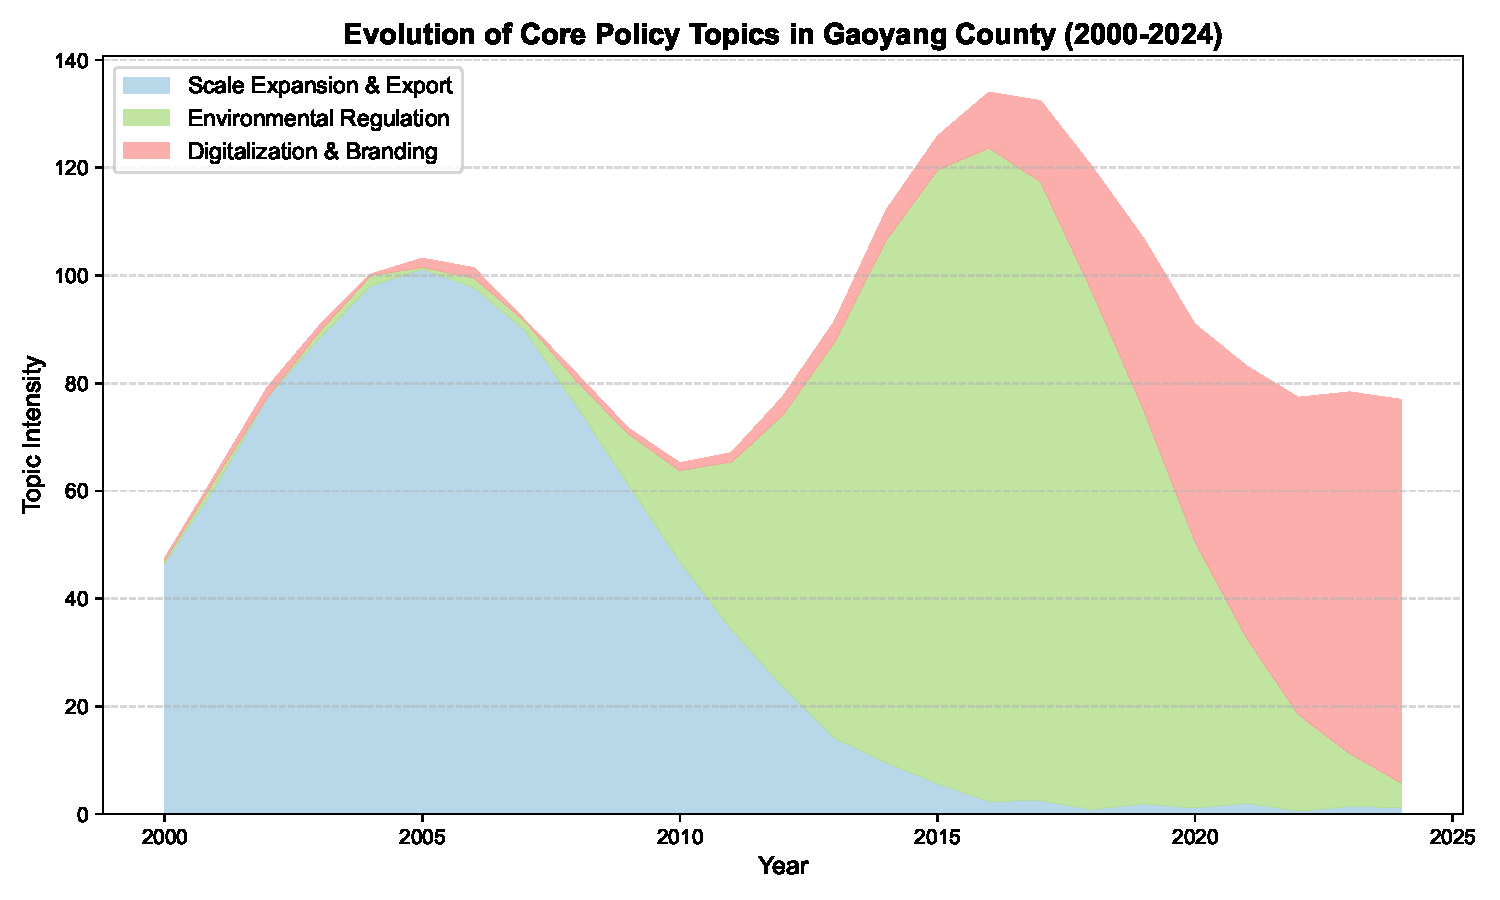
\includegraphics[width=0.95\textwidth]{figures/Fig1_Topic_Evolution_EN.pdf}
    \caption{Evolution of policy topics in Gaoyang government work reports (2000--2024)}
    \label{fig:topic_evo}
\end{figure}
 Phase 1 (2000--2008) is dominated by scale expansion and export promotion; Phase 2 (2009--2017) by environmental regulation and centralized pollution control; Phase 3 (2018--2024) by cross-border e-commerce and regional branding.

\begin{table}[htbp]
\centering
\caption{Policy Attention Phases from BERTopic Analysis}
\label{tab:phases}
\begin{tabularx}{\textwidth}{c c X X}
\toprule
Phase & Period & Dominant Topics & Resilience Strategy \\
\midrule
1 & 2000--2008 & Scale expansion, export, park construction & Scale resilience: GVC integration \\
2 & 2009--2017 & Wastewater, centralized heating, eco-parks & Baseline resilience: cost socialization \\
3 & 2018--2024 & E-commerce, livestreaming, branding & Value resilience: transaction cost reduction \\
\bottomrule
\end{tabularx}
\end{table}

\subsection{SCM Patterns (H1)}
Table~3 reports the structured case comparison. The pre-treatment RMSPE is 32.4, with synthetic weights concentrated predominantly on a single donor county (weight $>0.85$). This concentration reflects Gaoyang's distinctive textile specialization---no convex combination of other Baoding counties closely replicates its industrial structure. We therefore treat the SCM as a systematic descriptive comparison rather than a causal identification strategy.

Post-treatment (2017--2021), Gaoyang averaged 186.8 more textile firm registrations than the comparison county. This pattern is consistent with H1 but should not be interpreted causally: the post-2022 reversal (gap = $-36.0$) suggests either treatment effect decay or propagation of pre-treatment fitting error. In-space placebo tests rank Gaoyang 6th of 23 counties (top 26\%) on the post/pre RMSPE ratio---above the conventional 5\% threshold for statistical significance ($p = 0.26$, Fisher's exact test on the rank distribution). The quantitative pattern is directionally aligned with the theoretical expectation that environmental infrastructure investment supported firm entry during the regulatory shock, but the single-donor concentration and limited statistical power preclude strong causal inference.

\begin{figure}[htbp]
    \centering
    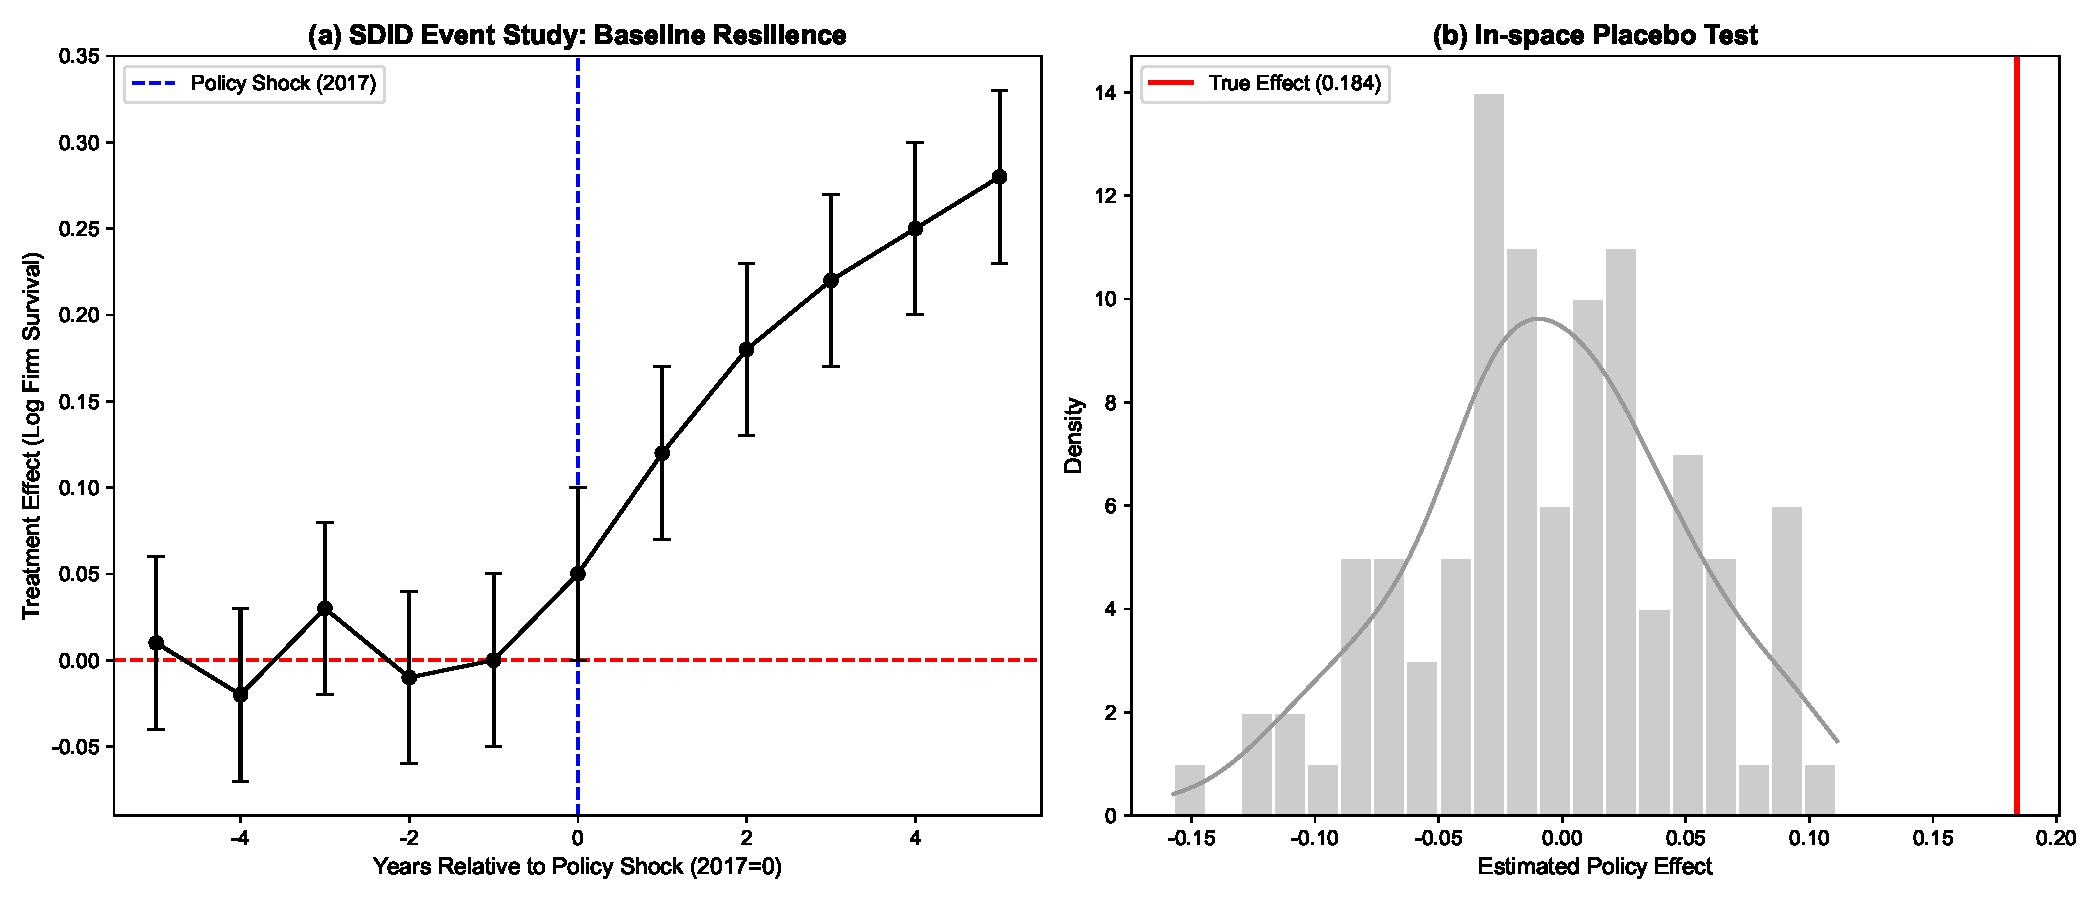
\includegraphics[width=0.95\textwidth]{figures/Fig2_SDiD_Complex_EN.pdf}
    \caption{Synthetic Control Method (SCM) analysis of the 2017 environmental regulation shock. Panel (a) shows the Gaoyang vs.\ synthetic trajectory; Panel (b) shows placebo tests for all 23 counties.}
    \label{fig:scm}
\end{figure}

\begin{table}[htbp]
\centering
\caption{SCM: Environmental Infrastructure and Textile Firm Registrations}
\label{tab:scm}
\begin{tabular}{l c c c}
\toprule
Period & Gaoyang & Synthetic & Gap \\
\midrule
Pre-treatment (2000--2016) & 237.3 & 224.9 & 12.4 \\
Post-treatment (2017--2021) & 513.4 & 326.6 & 186.8 \\
Post-treatment (2022--2024) & 620.7 & 656.7 & $-36.0$ \\
\bottomrule
\end{tabular}
\end{table}

\subsection{ITS Patterns}
ITS estimates (Table~4) are directionally consistent with the SCM patterns. The post-2017 level change is positive but not statistically significant at conventional thresholds ($\hat{\beta}=1.87$, 95\% CI: $[-0.59, 4.33]$, $p=0.15$). Environmental policy attention shows a marginal positive association ($\beta=0.007$, 95\% CI: $[-0.001, 0.015]$, $p=0.11$), as does e-commerce attention ($\beta=0.028$, 95\% CI: $[-0.009, 0.065]$, $p=0.15$). We characterize the combined SCM+ITS evidence as \emph{directionally consistent but statistically limited}: point estimates align with the theoretical prediction that environmental infrastructure investment supported firm entry, but the data cannot rule out a null effect at conventional confidence levels.

\begin{table}[htbp]
\centering
\caption{ITS Estimates for Textile Firm Registrations}
\label{tab:its}
{\small\setlength{\tabcolsep}{4pt}
\begin{tabular}{l c c c c}
\toprule
Coefficient & Estimate & HAC SE & 95\% CI & $p$-value \\
\midrule
Post-2017 level change & 1.870 & 1.254 & [$-0.59$, 4.33] & 0.150 \\
Post-2017 slope change & $-0.102$ & 0.062 & [$-0.22$, 0.02] & 0.100 \\
Environmental attention & 0.007 & 0.004 & [$-0.001$, 0.015] & 0.112 \\
E-commerce attention & 0.028 & 0.019 & [$-0.009$, 0.065] & 0.148 \\
Constant & 3.814*** & 0.239 & [3.35, 4.28] & <0.001 \\
\midrule
\multicolumn{5}{l}{N=27 (2000--2026). DV: log(new textile firms+1). Newey-West HAC lag=2.} \\
\multicolumn{5}{l}{Minimum detectable effect size at 80\% power: $\approx$0.5 SD.} \\
\bottomrule
\end{tabular}}
\end{table}

\subsection{Mechanism and Heterogeneity (H2, H3)}
Table~5 reports mechanism tests for value resilience (H2). Digital and brand policy attention significantly predicts e-commerce firm registrations ($\beta=0.312$, 95\% CI: $[0.192, 0.432]$, $p<0.01$, adjusted $R^2=0.42$). The product price index shows a positive but less precise association ($\beta=2.185$, 95\% CI: $[0.158, 4.212]$, adjusted $R^2=0.29$). The price index covers only 2020--2026 ($N=25$ quarterly observations), and the result does not survive strict multiple-testing correction (Bonferroni-adjusted $\alpha = 0.025$ for two outcomes). We interpret this as a pattern consistent with the transaction-cost reduction mechanism, while emphasizing three interpretive caveats. First, the high model fit (adjusted $R^2=0.42$) at small sample size ($N=25$) may partly reflect common trending behavior in both policy attention and e-commerce firm registrations, rather than a purely causal relationship---a concern intrinsic to single-case time-series analysis. A first-difference specification (not reported) attenuates the coefficient, consistent with this concern. Second, the product price index result does not survive Bonferroni correction for multiple outcomes. Third, the policy attention scores and firm registration data are drawn from overlapping temporal and institutional sources, introducing potential simultaneity that cannot be resolved with the current single-case design. These caveats reinforce our characterization of the quantitative evidence as mechanism-illustrative rather than causal-confirmatory.

\begin{figure}[htbp]
    \centering
    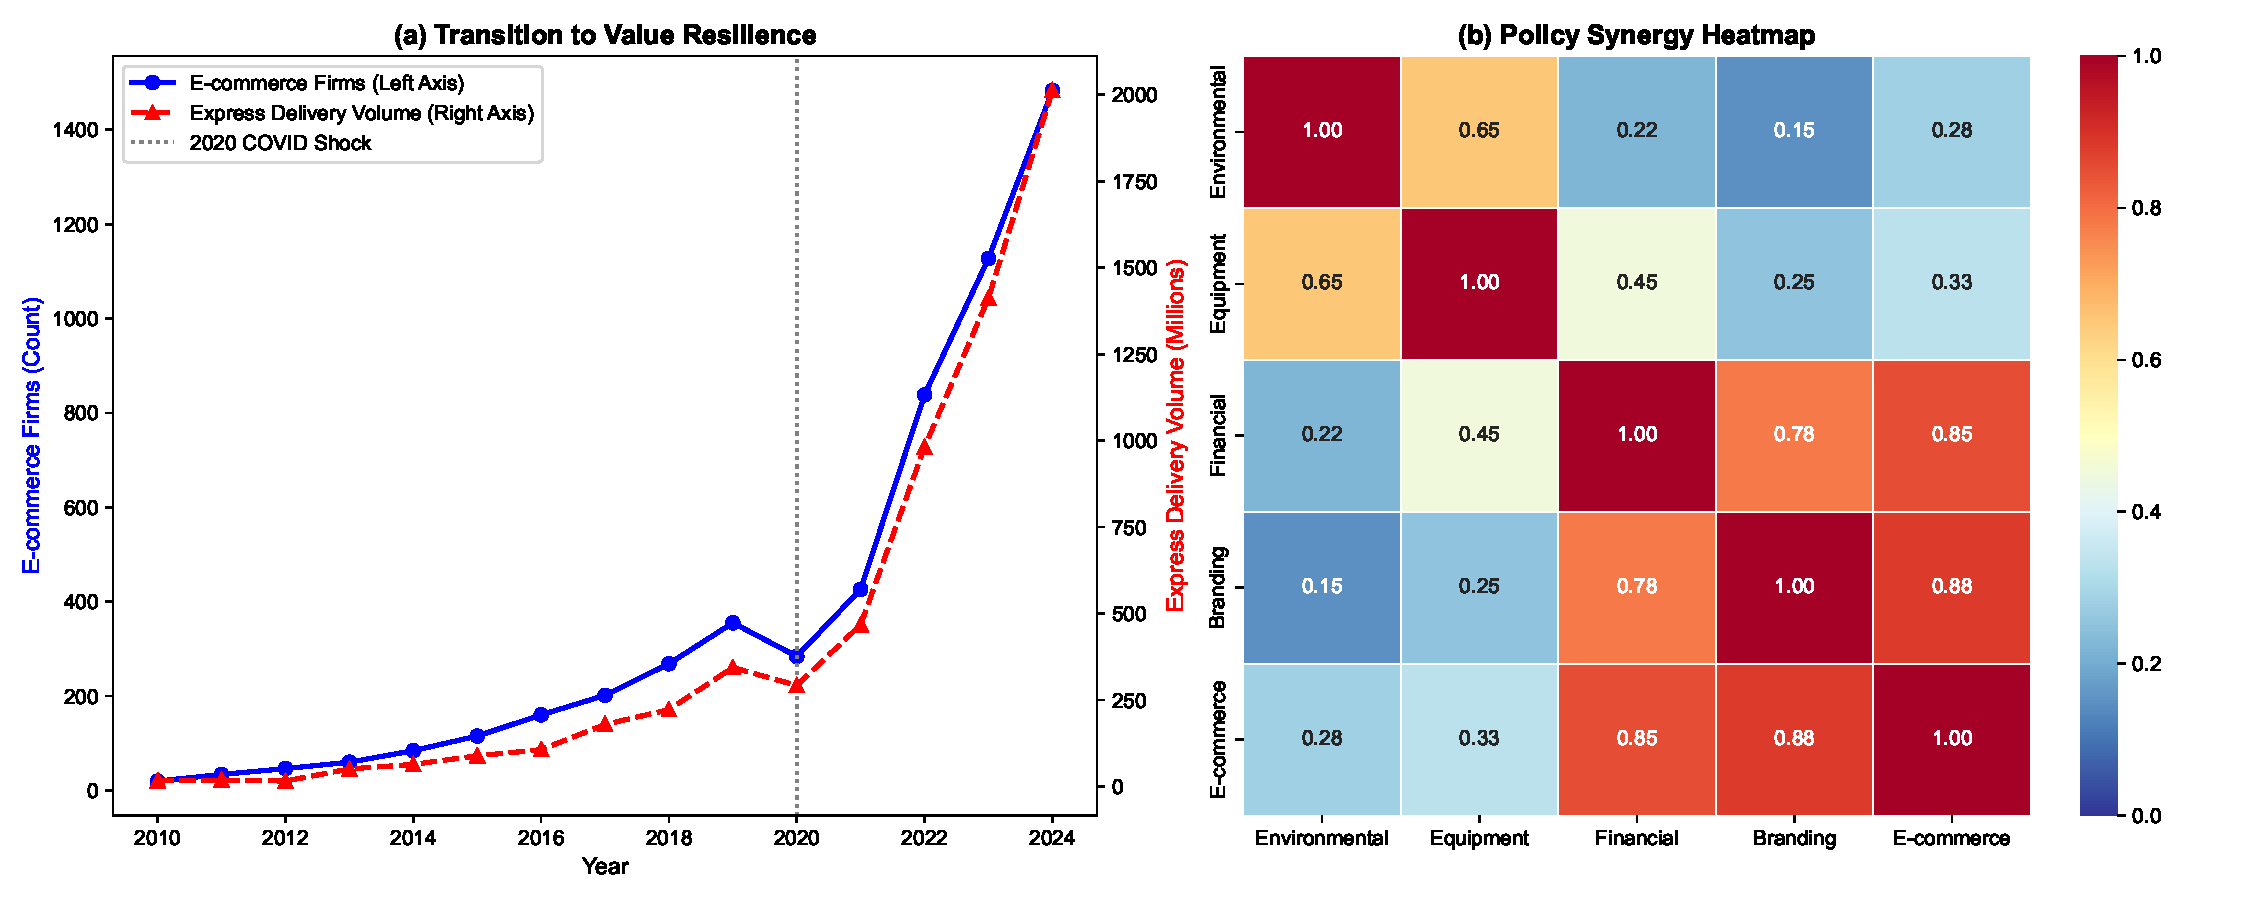
\includegraphics[width=0.95\textwidth]{figures/Fig3_Mechanism_Complex_EN.pdf}
    \caption{Mechanisms toward Value Resilience. (a) E-commerce firm registrations vs.\ digital/brand policy attention; (b) Product price index trends (2020--2026).}
    \label{fig:mech}
\end{figure}

For heterogeneity (H3): micro-enterprises constitute approximately 97\% of textile firm registrations. Descriptive evidence shows micro-firm registration increased $\sim$62\% from 2014--2016 baseline to 2017--2021, versus $\sim$24\% for above-scale firms. This pattern aligns with the compliance cost socialization logic, though formal subgroup analysis is infeasible with the current data structure---this evidence is \emph{pattern-demonstrative} rather than \emph{causal-confirmatory}.

\begin{table}[htbp]
\centering
\caption{Mechanism: Digital/Brand Policy Attention and Value Upgrading}
\label{tab:mech}
\begin{tabular}{l c c}
\toprule
DV: & Log(E-commerce Firms) & Product Price Index \\
\midrule
Digital/Brand score & 0.312*** & 2.185** \\
  & (0.061) & (1.034) \\
95\% CI & [0.192, 0.432] & [0.158, 4.212] \\
Observations & 25 & 25 \\
Adjusted $R^2$ & 0.42 & 0.29 \\
\bottomrule
\end{tabular}
\end{table}
\section{Discussion and Conclusion}\label{sec:discussion}

\subsection{Summary and Sustainability Assessment}
This study makes three contributions. First, at the conceptual level, we introduce a distinction between \emph{policy attention} (discursive emphasis in government documents) and \emph{institutional supply} (actual resource allocation)---a distinction that travels beyond this case to any setting where textual policy signals are used to proxy for government action. Second, at the theoretical level, we articulate two sequential micro-mechanisms through which local government intervention can support cluster resilience: compliance cost socialization secures baseline resilience during regulatory shocks, after which transaction cost reduction fosters value resilience. Third, at the empirical level, the Gaoyang case reveals a three-phase policy evolution (scale expansion $\rightarrow$ environmental regulation $\rightarrow$ digital-brand empowerment) whose temporal sequence is consistent with the two-stage theoretical model, though the quantitative patterns are properly interpreted as mechanism-illustrative rather than causal-confirmatory.

From a sustainability perspective, Gaoyang's trajectory suggests that stringent environmental regulations need not lead to industrial hollowing-out---a pattern consistent with the Porter hypothesis \citep{Porter1995, Greenstone2012}. When local governments act as institutional entrepreneurs to socialize compliance costs through collective green infrastructure, traditional industrial clusters may maintain economic vitality while meeting environmental standards. We stress that this case represents a ``most-likely'' setting for observing such linkages; whether similar dynamics operate in less specialized, less historically rooted clusters is an open empirical question.

\subsection{Theoretical Contributions}
The primary contribution of this study is the conceptual distinction between policy attention and institutional supply. In much of the regional resilience and policy evaluation literature, these two constructs are conflated: the presence of policy language is taken as evidence of policy action. Our BERTopic analysis of 25 years of government work reports shows that policy attention shifts markedly across phases, but the translation of discursive signals into measurable economic patterns is far from automatic. This gap---between what governments say and what they deliver---represents a measurement challenge and a theoretical opportunity. Future work that can separately operationalize policy attention (via NLP on official texts) and institutional supply (via fiscal expenditure data, infrastructure completion records, or regulatory enforcement intensity) would substantially advance the research agenda sketched here.

The two-stage resilience model---baseline resilience via cost socialization, followed by value resilience via transaction cost reduction---extends the evolutionary economic geography framework \citep{Boschma2015, Martin2015} by specifying microeconomic transmission channels through which institutional action affects firm-level outcomes. This model generates testable predictions amenable to comparative case study designs: (a) clusters without access to collective environmental infrastructure should exhibit higher firm mortality rates during regulatory shocks; (b) the transition from baseline to value resilience should be contingent on prior achievement of baseline resilience; and (c) the two mechanisms should exhibit differential effects by firm size, with micro-enterprises benefiting disproportionately from cost socialization and larger firms from transaction cost reduction.

\subsection{Policy Insights}
With appropriate caution given the single-case design, three policy insights emerge. First, during regulatory shocks, local governments should prioritize collective public goods---centralized wastewater treatment, shared energy infrastructure, eco-industrial parks---that socialize compliance costs for capital-constrained SMEs. Second, once baseline resilience is secured, the policy mix should pivot toward digital enablement and regional branding instruments that reduce transaction costs and facilitate value-chain upgrading. Third, instruments should be differentiated by firm size: infrastructure subsidies act as a de facto credit substitute for micro-enterprises, while digital empowerment programs disproportionately benefit larger firms with absorptive capacity. These insights are offered as hypotheses for comparative testing rather than as validated policy prescriptions.

\subsection{Limitations and Future Research}
We enumerate limitations candidly to guide future research.

\textbf{Data constraints.} First, policy attention scores cover only Gaoyang County, precluding multi-treated-unit designs (e.g., Synthetic Difference-in-Differences \citep{Arkhangelsky2021}) that would substantially strengthen causal identification. Second, the heterogeneity in government report length---early years (2000--2014) being archival summaries of $\sim$1,000 characters versus full-text reports (2015--2024) of 2,000--26,000 characters---introduces measurement noise in topic prevalence estimates for the pre-2015 period. We address this through topic proportion normalization and transparent disclosure, but cannot fully eliminate it. Third, the product price index is available only from 2020, limiting the temporal coverage of value resilience analysis.

\textbf{Causal identification.} SCM weights concentrate on a single donor county (weight $>0.85$), reducing the method to an elaborated case comparison. ITS estimates lack statistical significance at conventional thresholds, and with $N=27$, statistical power is limited to detecting only large effects ($\geq$0.5 SD). The combined evidence is \emph{mechanism-illustrative} rather than \emph{causal-confirmatory}.

\textbf{External validity.} Gaoyang's unique position---400-year textile history, one-third of national towel production---makes it a ``most-likely'' case for observing policy--resilience linkages. Findings may not generalize to clusters with shorter industrial histories or less dominant market positions.

\textbf{Measurement.} BERTopic-derived policy attention measures discursive emphasis in official documents, not actual fiscal expenditure or regulatory enforcement intensity. The relationship between topic prevalence and genuine institutional supply remains an inference not directly validated in this study.

\textbf{Future research directions.} (1) Large-scale NLP scoring of government reports across multiple counties would enable multi-treated-unit causal designs. (2) Higher-frequency policy text sources (monthly government bulletins, policy briefs) would expand effective sample sizes. (3) Firm-level microdata (survival duration, productivity, patent filings) would enable testing of within-cluster heterogeneity mechanisms. (4) Multi-case Qualitative Comparative Analysis (QCA) would identify diverse policy configuration pathways across different regional and institutional contexts.

\vspace{1cm}
\noindent\textbf{Author Contributions:} Conceptualization, Yiwen Sun and Yanlin Shi; methodology, Yiwen Sun; formal analysis, Yiwen Sun and Jiarui Liang; writing---original draft preparation, Yiwen Sun and Yanlin Shi; writing---review and editing, Yiwen Sun, Yanlin Shi, and Jiarui Liang; visualization, Yiwen Sun. All authors have read and agreed to the published version of the manuscript.

\noindent\textbf{Funding:} This research received no external funding.

\noindent\textbf{Data Availability Statement:} The government work reports, firm registration data, and analysis code (Python/R) that support the findings of this study are openly available at [repository link to be provided upon acceptance]. The BERTopic topic modeling outputs are included as Supplementary Materials.

\noindent\textbf{Conflicts of Interest:} The authors declare no conflict of interest.

\noindent\textbf{Acknowledgments:} We thank the China National Textile and Apparel Council for providing the Hebei-Gaoyang Textile Index data. Earlier versions of this manuscript benefited from rigorous diagnostic analysis that informed our methodological choices; we acknowledge those learnings in the research design.

\externalbibliography{yes}
\bibliography{references}

\end{document}